\documentclass[t,compress,aspectratio=169]{beamer}

\beamertemplatenavigationsymbolsempty

\usepackage[utf8x]{inputenc}
\usepackage{beamerthemeAir}
\usepackage{bookman}
% \beamertemplateballitem

%\usepackage[svgnames]{xcolor}
\usepackage{listings}
\usepackage{color}
\definecolor{lightgray}{rgb}{.9,.9,.9}
\definecolor{darkgray}{rgb}{.4,.4,.4}
\definecolor{purple}{rgb}{0.65, 0.12, 0.82}

\lstset{
    language=C++,
    frame=lines,
    breaklines=true,
    tabsize=4,
    extendedchars=true,
    columns=fixed,
    numbers=left,
    stepnumber=1,
    numbersep=5pt,
    numberstyle=\scriptsize,
    basicstyle=\ttfamily\scriptsize,
    keywordstyle=\color{blue}, % \color{blue}
    identifierstyle={\color{Black}},
    commentstyle=\color{Green},
    stringstyle=\color{red},
    backgroundcolor={\color{white}},
    showstringspaces=false,
    morekeywords = {
        Q_OBJECT, Q_PROPERTY, Q_INTERFACES, Q_SLOTS, Q_SIGNALS, foreach, qobject_cast
        }
}

\lstdefinelanguage{JavaScript}{
  keywords={typeof, new, true, false, catch, function, return, null, catch, switch, var, if, in, while, do, else, case, break},
  keywordstyle=\color{blue}\bfseries,
  ndkeywords={class, export, boolean, throw, implements, import, this},
  ndkeywordstyle=\color{darkgray}\bfseries,
  identifierstyle=\color{black},
  sensitive=false,
  comment=[l]{//},
  morecomment=[s]{/*}{*/},
  commentstyle=\color{purple}\ttfamily,
  stringstyle=\color{red}\ttfamily,
  morestring=[b]',
  morestring=[b]"
}
\lstset{
    language=JavaScript,
%    frame=lines,
    breaklines=true,
    tabsize=4,
    extendedchars=true,
    columns=fixed,
    numbers=left,
    stepnumber=1,
    numbersep=5pt,
    numberstyle=\scriptsize,
    basicstyle=\ttfamily\scriptsize,
%     keywordstyle=\color{blue},
%     identifierstyle={\color{black}},
%     commentstyle=\color{green},
%     stringstyle=\color{red},
%     backgroundcolor={\color{white}},
    showstringspaces=false,
}
\usepackage{algorithmicx}
\usepackage{multirow}
\usepackage{pdfpages}

\usepackage{soul}
\renewcommand<>{\hl}[1]{\sethlcolor{airlightblue}\only#2{\beameroriginal{\hl}}{#1}}
\makeatletter
\newcommand\SoulColor{%
  \let\set@color\beamerorig@set@color
  \let\reset@color\beamerorig@reset@color}
\makeatother
\SoulColor

\setbeamercovered{dynamic}

\AtBeginSection[] {
\begin{frame}<beamer>
\frametitle{Next up...}
\tableofcontents[currentsection]
\end{frame}}

\makeatletter
    \newenvironment{withoutheadline}{
        \setbeamertemplate{headline}{\vskip \headheight}
    }{}
\makeatother


\setbeamertemplate{title page}{%
\noindent

\vspace{.25\textheight}

\centering
{\huge\bfseries\textcolor{airdarkblue}{\inserttitle}}

\vspace{.1\textheight}

\noindent\centering
{\large\insertsubtitle}

\vspace{.4\textheight}

\noindent
\begin{minipage}{.5\textwidth}
 \insertauthor
\end{minipage}%
\begin{minipage}{.5\textwidth}
 \begin{flushright}
  \href{mailto:\authoremail}{\authoremail}
 \end{flushright}
\end{minipage}

}



\title{SPDX License Markers in KDE}
\subtitle{Progress Update}
\author{Andreas Cord-Landwehr}
\newcommand{\authoremail}{cordlandwehr@kde.org}

\lstset{ %
  language=C++,
%   backgroundcolor=\color{KDEgray4},
%   basicstyle=\footnotesize\ttfamily,
%   breakatwhitespace=false,
%   breaklines=true,
%   captionpos=b,
%   commentstyle=\color{KDEgreen},
%   escapeinside={\%*}{*)},
%   extendedchars=true,
%   frame=single,
%   keywordstyle=\color{KDEblue},
%   language=Prolog,
%   numbers=left,
%   numbersep=5pt,
%   numberstyle=\tiny\color{lightgray},
%   rulecolor=\color{lightgray},
%   showspaces=false,
%   showstringspaces=false,
%   showtabs=false,
%   stepnumber=1,
%   stringstyle=\color{KDEorange},
%   tabsize=2,
%   title=\lstname,
  morekeywords={Item,import,not,\},\{,Q_SIGNALS,public,Q_OBJECT,virtual,NOTIFY,Q_NULLPTR,Q_DISABLE_COPY,Q_DECL_OVERRIDE},
%   deletekeywords={time}
}

\begin{document}

\usebackgroundtemplate{
\includegraphics[height=\paperheight]{1920x1080-akademy}}
\begin{withoutheadline}
\begin{frame}
\titlepage
\end{frame}
\end{withoutheadline}
\usebackgroundtemplate{
\includegraphics[height=\paperheight]{1920x1080-noakademy}}

%==============================================================================

\begin{frame}
    {What is a License?}

    Via copyright, your work is not reusable by anybody else -- a license changes this

    \begin{description}
        \item [License] defines under which terms your software can be reused
        \item [Free Software License] must grant the following 4 rights:
            \begin{enumerate}
                \item Use
                \item Study
                \item Share
                \item Improve
            \end{enumerate}
        \item [Copyleft license] requires that same rights preserve in derivative works\\ (e.g. GPL, LGPL)
        \item [Permissive license] only minimal restrictions of 4 freedoms, but no requirements for derivative works (e.g. BSD, MIT)
    \end{description}
\end{frame}

\begin{frame}[fragile]
    {License Statements since the 80s -- The old way}

    \begin{example}[Example of Traditional License Header]
    \tiny
    \begin{verbatim}
    /*
        This file is part of Rocs.
        Copyright 2008-2011  Tomaz Canabrava <tomaz.canabrava@gmail.com>
        Copyright 2008       Ugo Sangiori <ugorox@gmail.com>
        Copyright 2010       Wagner Reck <wagner.reck@gmail.com>
        Copyright 2014       Andreas Cord-Landwehr <cordlandwehr@kde.org>

        This program is free software; you can redistribute it and/or
        modify it under the terms of the GNU General Public License as
        published by the Free Software Foundation; either version 2 of
        the License, or (at your option) any later version.

        This program is distributed in the hope that it will be useful,
        but WITHOUT ANY WARRANTY; without even the implied warranty of
        MERCHANTABILITY or FITNESS FOR A PARTICULAR PURPOSE.  See the
        GNU General Public License for more details.

        You should have received a copy of the GNU General Public License
        along with this program.  If not, see <https://www.gnu.org/licenses/>.
    */
    \end{verbatim}
    \end{example}
\end{frame}

\pgfdeclareimage[height=.1\paperheight]{pageheader}{categories/thumbsup.jpg}
\begin{frame}[fragile]
    {License Statements Today}

    \begin{example}[REUSE Compatible License Statement]
    \tiny
    \begin{verbatim}
    /*
        This file is part of Rocs.
        SPDX-FileCopyrightText: 2008-2011 Tomaz Canabrava <tomaz.canabrava@gmail.com>
        SPDX-FileCopyrightText: 2008 Ugo Sangiori <ugorox@gmail.com>
        SPDX-FileCopyrightText: 2010 Wagner Reck <wagner.reck@gmail.com>
        SPDX-FileCopyrightText: 2014 Andreas Cord-Landwehr <cordlandwehr@kde.org>

        SPDX-License-Identifier: GPL-2.0-or-later
    */
    \end{verbatim}
    \end{example}
    
    \begin{itemize}
        \item Easier to read
        \item Hard to make errors in statements
        \item Enables automatic tooling for checking
        \item Decided to be KDE's new way for license statements
    \end{itemize}

\end{frame}

\pgfdeclareimage[height=.1\paperheight]{pageheader}{reuse.png}
\begin{frame}
    {Where to find more about REUSE in KDE}

    \begin{itemize}
        \item SPDX is a specification, written by legal experts:\\
            \url{https://spdx.github.io/spdx-spec/}
        \item \url{https://REUSE.software} is initiative by FSFE to make reusing easier
        \item Provide a simple specification that requires only tiny subset and gives guidelines how to apply it
        \item In a nutshell:
            \begin{enumerate}
                \item Add SPDX-License-Identifier tag to every file
                \item Add SPDX-FileCopyrightText tag to every file
                \item Add license text in \texttt{LICENSES/<license>.txt} for every license
            \end{enumerate}
        \item See KDE Licensing HowTo Wiki page: \url{https://community.kde.org/Guidelines_and_HOWTOs/Licensing}
    \end{itemize}
\end{frame}

\begin{frame}
    {Statistics 1/4}
    {Frameworks are done!}
    
    \begin{center}
        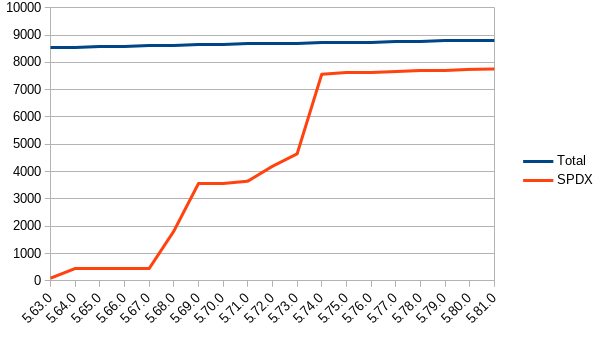
\includegraphics[height=.6\paperheight]{kde-frameworks}
    \end{center}
    
    Remaining ones are deprecated
\end{frame}

\begin{frame}
    {Statistics 2/4}
    {Plasma is following strong}
    
    \begin{center}
        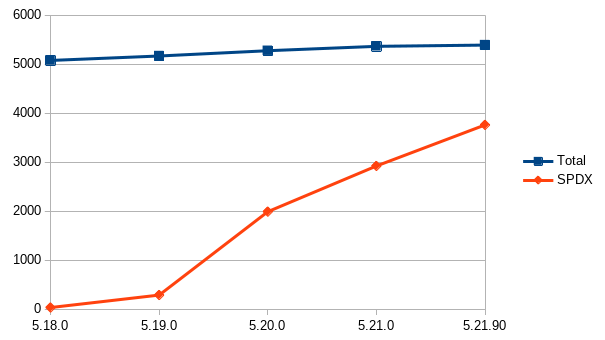
\includegraphics[height=.6\paperheight]{plasma}
    \end{center}
\end{frame}


\begin{frame}
    {Statistics 3/4 : Current Status (cpp \& h)}
    {39.515 out of 67.039 files = 58.94\,\% !!!}
    
    \begin{center}
        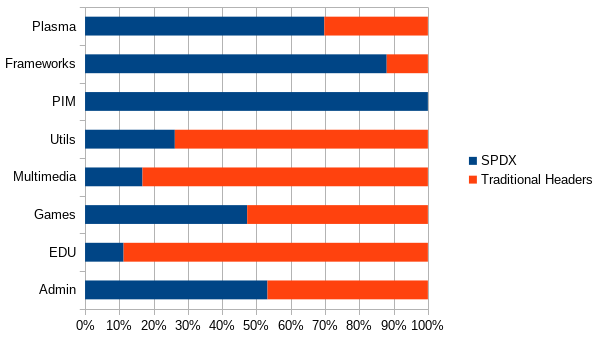
\includegraphics[height=.68\paperheight]{overall}
    \end{center}
\end{frame}

\begin{frame}
    {Statistics 4/4 : License Statistics for all KDE Code}
    {Disclaimer: Only SPDX marked files included \& only licenses that are used $> 10$ times}
    
    \vspace{-1.5em}
    \begin{center}
        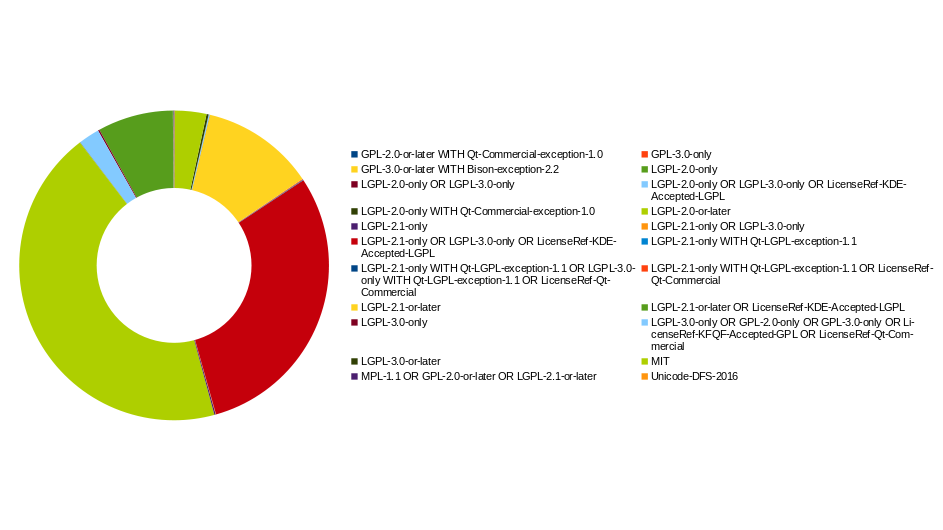
\includegraphics[height=.7\paperheight]{license-overview}
    \end{center}
    \vspace{-2em}
    
    Note: Currently, there are 53 different license statements in the code base.
\end{frame}

\begin{frame}
    \frametitle{The End}
    \vspace{0.3cm}
    \begin{block}{}
        \centering\begin{Huge}Convert your project today :)\end{Huge}
    \end{block}
    \medskip
    \textbf{Thanks to all who are helping! It is great to see so many people involved!}

    \vspace{0.5cm}
    \begin{tiny}
        \begin{block}{Easy Steps to Follow}
            \begin{description}
                \item [KDE License HowTo] \url{https://community.kde.org/Guidelines_and_HOWTOs/Licensing}
                \item [Licensedigger] KDE conversion tooling: \url{https://invent.kde.org/sdk/licensedigger}
                \item [Support] irc: CoLa, mail: \url{cordlandwehr@kde.org}
            \end{description}
        \end{block}
    \end{tiny}
\end{frame}

\end{document}
